\chapter{Nástroje pre sieťovú virtualizáciu}
\label{chap:nastroje_pre_siet_virt}

V tejto kapitole uvádzam prehľad momentálne dostupných nástrojov virtuálnych sieťových laboratórii. Používaniu jednotlivých riešení sa budem venovať v kapitole \ref{chap:analyza_vyucovania} - \nameref{chap:analyza_vyucovania}.
  
\section{Porovnávacie kritériá}

Pri porovnávaní jednotlivých virtuálnych sieťových laboratórii som sa rozhodoval podľa nasledovných kritérii:
\begin{itemize}
    \item Použité vývojové technológie
    \item Podpora zariadení
    \item Typ používateľského rozhrania
    \item Prideľovanie portových čísel zariadeniam
    \item Vzdialený prístup ku zariadeniam (telnet, vnc, rdp)
    \item Vytvorenie/úprava/uloženie/odstránenie topológie
    \item Počet topológii, ktoré môže mať jeden používateľ spustených
    \item Možnosť práce viac ľudí naraz na rovnakom projekte
    \item Možnosť prepojiť topológiu so živou sieťou
    \item Vývoj nástroja v budúcnosti
    \item Vybrané výhody a nevýhody nástroja
\end{itemize}


\section{Dostupné riešenia}

\subsection{Cisco Packet Tracer}

Cisco Packet Tracer je, ako je zrejmé z názvu, nástroj na vizualizáciu sietí vyvíjaný spoločnosťou Cisco. Je vhodný na uvedenie do problematiky sieťových technológii. Nevýhodou je, že nie je open-source a je prístupný výlučne pre členov \emph{Cisco Networking Academy}. Na druhej strane je vyvíjaný pre platformy Windows a Linux, po emulácii aj na macOS \cite{packet_tracer_mac}. Ďalšou výhodou je podpora mobilných platforiem prostredníctvom aplikácie \emph{Packet Tracer Mobile}. Slúži na emuláciu jednoduchých aktívnych aj pasívnych sieťových prvkov a jednoduchých koncových zariadení \cite{packet_tracer}. Čo sa týka smerovačov a prepínačov, tieto sú podporované, ale iba Cisco s obmedzenou funkcionalitou. Nie je možné ho ďalej rozširovať ani funkcionálne, ani ďalšími zariadeniami napr. o zariadenia iných výrobcov alebo koncové stanice Linux/Windows.

Nástroj Packet Tracer je možné používať výlučne lokálne, pretože pre tento nástroj neexistuje serverové riešenie. Vzdialený prístup a vytváranie topológii sa realizuje prostredníctvom grafického rozhrania aplikácie. Topológie si spravuje sám používateľ aplikácie. Nástroj nevie rozlišovať rôzne typy používateľov. Je nenáročný na systémové zdroje. Umožňuje pracovať súčasne iba s jednou topológiou, ktorú je možné kedykoľvek zavrieť. Topológiu nástroj nie neumožňuje prepojiť so živou sieťou.

Na obrázku \ref{obr:packet_tracer} je znázornený nástroj Dynagen.

\begin{figure}
    \centering
    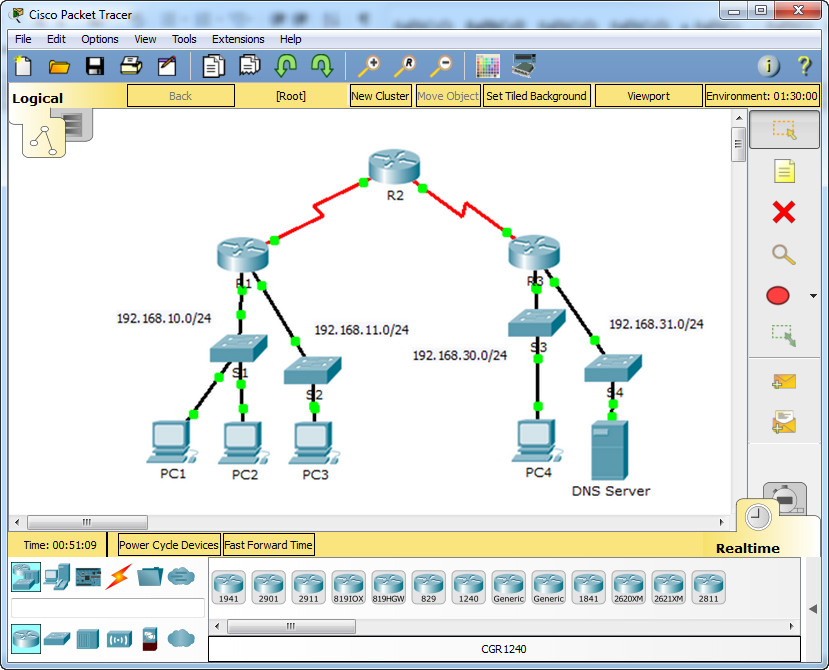
\includegraphics[width=0.75\textwidth]{packet_tracer}
    \caption{Nástroj Cisco Packet Tracer spustený v prostredí Windows}
    \cite{obr_packet_tracer}
    \label{obr:packet_tracer}
\end{figure}

\subsection{Dynamips/Dynagen}

Dynamips je open-source emulátor Cisco smerovačov na Linux/Windows \cite{dynamips}. Nástroj je v prevažnej mierie napísaný v jazyku C \cite{dynamips_github}. Podporuje iba výlučne vybrané Cisco smerovače \cite{dynamips}. Ovláda sa cez príkazový riadok. Portové čísla na vzdialený prístup sa zariadeniam prideľujú manuálne. Vzdialený prístup k zariadeniam v topológii je realizovaný protokolom \emph{telnet}. Na vytváranie topológii sa používa jednoduchý značkovací jazyk.

Nástroj Dynagen, ktorý slúži ako nadstavba nad platformou Dynamips, slúži na jednoduchšiu prácu s topológiami \cite{dynamips}. Topológie môže spravovať výlučne administrátor, pretože ani Dynamips, ani Dynagen nevedia rozlišovať rôzne typy používateľov. Počet topológii, ktoré môžu byť súčasne spustené je obmedzené iba výkonom servera. Na jednej topológii môžu pracovať aj viacerí študenti, tým že sa rozdelia portové čísla zariadení v topológii medzi študentov. Nástroj Dynamips umožňuje prepojiť topológiu so živou sieťou \cite{dynamips, dynamips_nil}. 

V súčasnosti sa o nástroj starajú vývojári nástroja GNS3 \cite{dynamips_github}. Na obrázku \ref{obr:dynamips_dynagen} je znázornený nástroj Dynagen.

\begin{figure}
    \centering
    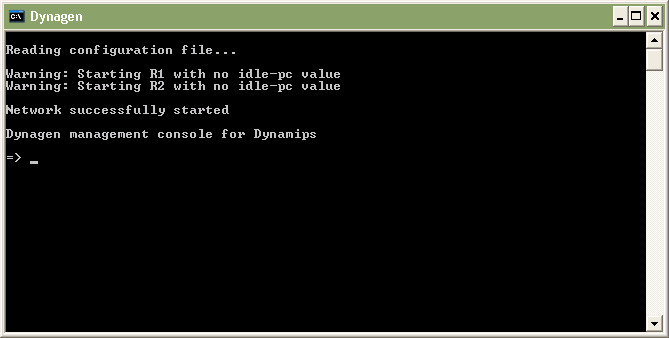
\includegraphics[width=0.75\textwidth]{dynamips_dynagen}
    \caption{Nástroj Dynagen spustený v prostredí Windows} \cite{obr_dynamips_dynagen}
    \label{obr:dynamips_dynagen}
\end{figure}

\subsection{WEB-IOU}

WEB-IOU, je simulačný nástroj pre platformu Linux, ktorý podporuje výlučne Cisco IOU platformu. Jeho hlavnou výhodou je podpora Cisco prepínačov, ktorá pri Dynamips/Dynagen chýba. Jeho autorom je Andrea Dainese \cite{webiou_github, webiou_unetlab_unetlabv2}.Nástroj je v prevažnej mierie napísaný v jazykoch PHP a JavaScript \cite{webiou_github}. Podporuje iba výlučne vybrané Cisco smerovače na platforme IOU - IOS on Unix \cite{webiou_firewall_cx}. Je vhodný na trénovanie pri certifikáciách CCNP a do istej miery aj CCIE. 

Spravuje sa cez príkazový riadok. Používateľovi je dostupné web rozhranie. Portové čísla na vzdialený prístup sa zariadeniam prideľujú automaticky. Vzdialený prístup k zariadeniam v topológii je realizovaný protokolom \emph{telnet}. Na vytváranie topológii sa používa jednoduchý značkovací jazyk \emph{NETMAP}. Topológie môže ktokoľvek, kto má prístup k web rozhraniu, pretože ani tento nástroj nevie rozlišovať rôzne typy používateľov. Počet topológii, ktoré môžu byť súčasne spustené je obmedzené iba výkonom servera. Napriek tomu môžu na jednej topológii môžu pracovať aj viacerí študenti rovnakým spôsobom, ako pri nástroji Dynamips/Dynalab. Nástroj WEB-IOU tiež umožňuje prepojiť topológiu so živou sieťou \cite{webiou_real_network}. 

V súčasnosti sa už nástroj nevyvíja. Na obrázku \ref{obr:webiou} je znázornené webové rozhranie nástroja WEB-IOU.

\begin{figure}
    \centering
    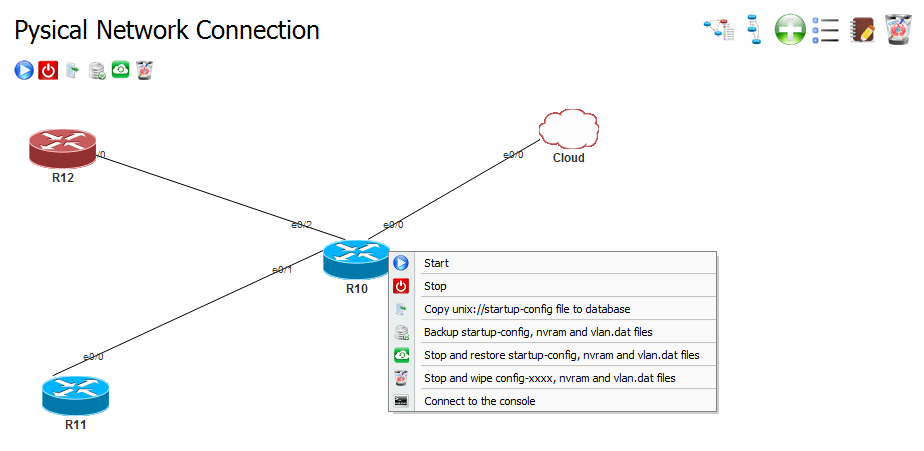
\includegraphics[width=0.75\textwidth]{webiou}
    \caption{Webové rozhranie nástroja WEB-IOU} \cite{obr_webiou}
    \label{obr:webiou}
\end{figure}

\subsection{Cisco VIRL}

VIRL, Virtual Internet Routing Lab, je komerčný simulačný nástroj sietí vyvíjaný spoločnosťou Cisco. Podporuje nielen Cisco smerovače a prepínače, ale aj zariadenia iných výrobcov, hoci ich integrácia nemusí byť jednoduchá. Výhodou oproti iným nástrojom je možnosť pridať podporované zariadenia do topológie ako LXC kontajner. Nevýhodou je, že nepodporuje Dynamips/Dynagen emuláciu, takže na ňom nie je možné využiť existujúce virtuálne zariadenia na katedre. Nástroj je postavený na platforme Linux (Debian) a je dostupný ako virtuálny stroj pre rôzne platformy. Je vhodný na trénovanie pri certifikáciách CCNP a do istej miery aj CCIE \cite{virl_cisco}. 

Spravuje sa cez príkazový riadok. Používateľovi je dostupné web rozhranie. Portové čísla na vzdialený prístup sa zariadeniam prideľujú automaticky \cite{virl_interfacett_1}. Vzdialený prístup k zariadeniam v topológii je realizovaný protokolmi \emph{telnet} a \emph{ssh}, po úprave aj \emph{vnc} \cite{virl_ciscoskills, virl_speaknetworks}. Na vytváranie topológii sa používa Nástroj \emph{VM Maestro}. Ten poskytuje možnosť, vopred si nakonfigurovať zariadenie podľa zvolených scenárov pomocou funkcie \emph{AutoNetkit}. Aj napriek tomu, že VIRL poskytuje pomerne podrobné možnosti na konfiguráciu zariadení a topológii, jeho používanie je pomerne obtiažne, hlavne pri vytváraní topológii \cite{virl_interfacett_1, virl_interfacett_2}. Cisco VIRL vie rozlišovať rôzne typy používateľov \cite{virl_cisco_features}. Počet topológii, ktoré môžu byť súčasne spustené je obmedzené iba výkonom servera. Napriek tomu môžu na jednej topológii môžu pracovať aj viacerí študenti rovnakým spôsobom, ako pri nástroji Dynamips/Dynalab \cite{virl_interfacett_2}. Nástroj tiež umožňuje prepojiť topológiu so živou sieťou \cite{virl_speaknetworks}. 

Nástroj v súčasnosti existuje iba vo verzii \emph{Personal Edition} s licenciou na 20 zariadení, čo výrazným spôsobom obmedzuje jeho využitie pri vyučovaní. V minulosti existovali aj verzie \emph{Personal Edition} s licenciou na 30 zariadení a \emph{Academic Edition}. Rozdiel medzi Personal a Academic Edition bol iba ten, že Academic Edition bol prístupný učiteľom a študentom za výhodnejšiu cenu. Podporované funkcionality boli zhodné v oboch verziách \cite{virl_edition_differences}. Na obrázkoch \ref{obr:virl_vmmaestro} a \ref{obr:virl_web} je v tomto poradí znázornený nástroj na vytváranie topológii VM Maestro a webové rozhranie Cisco VIRL.

\begin{figure}
    \centering
    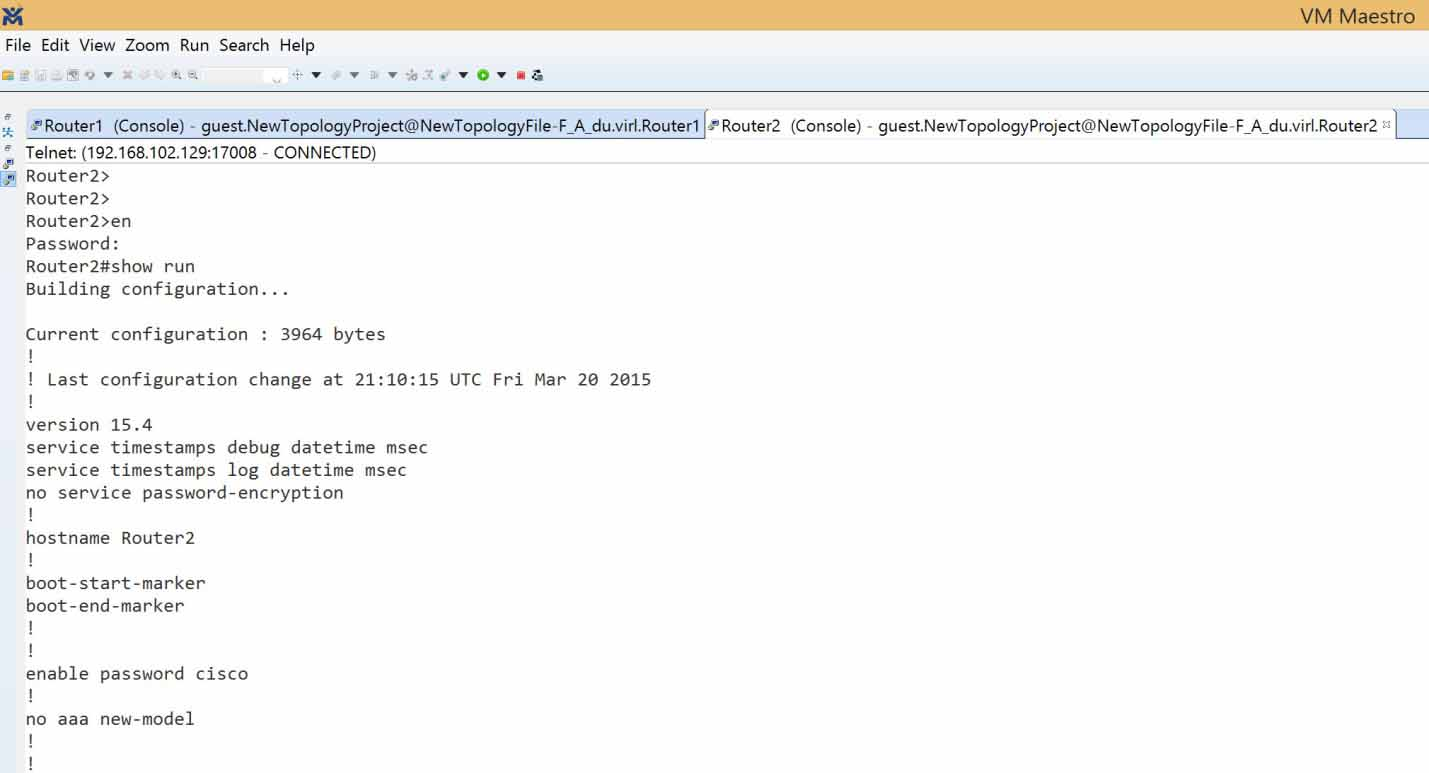
\includegraphics[width=0.75\textwidth]{virl_vmmaestro}
    \caption{VM Maestro} \cite{obr_virl_vmmaestro}
    \label{obr:virl_vmmaestro}
\end{figure}

\begin{figure}
    \centering
    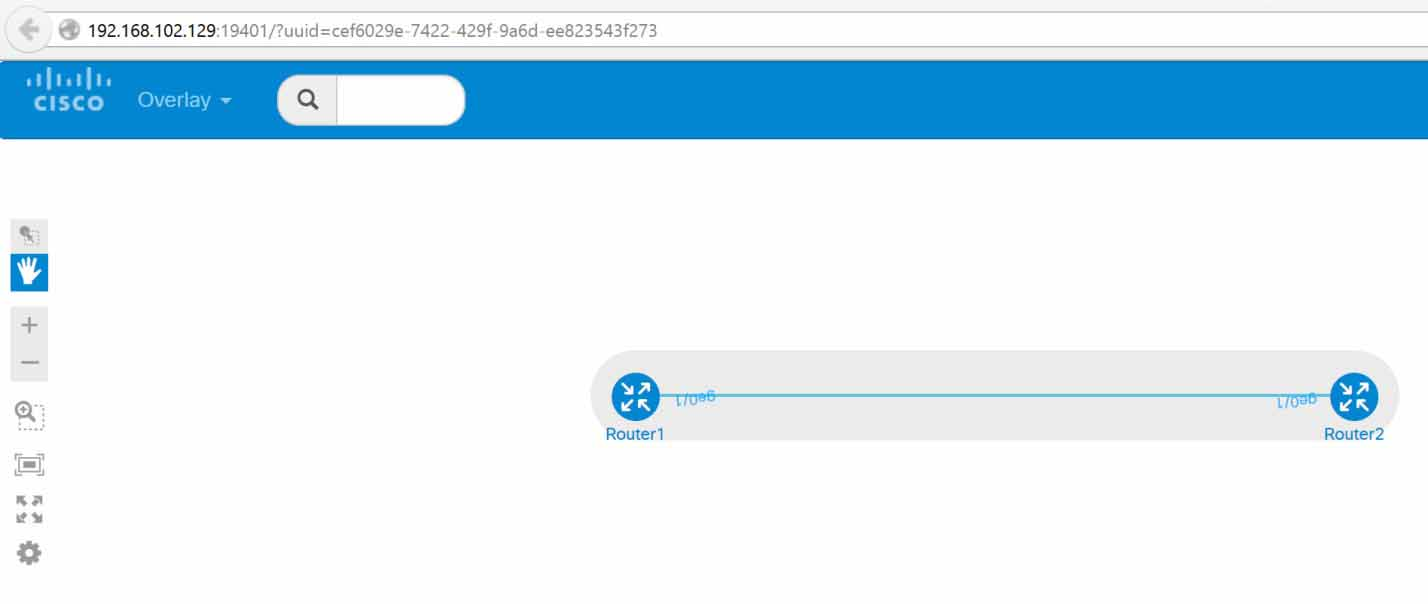
\includegraphics[width=0.75\textwidth]{virl_web}
    \caption{Cisco VIRL web rozhranie} \cite{obr_virl_web}
    \label{obr:virl_web}
\end{figure}

\subsection{ViRo v2}

ViRo, resp. ViRo v2, je virtuálne laboratórium vytvorený na Katedre informačných sietí. Nástroj vznikol ako výsledok diplomovej práce Ing. Petra Hadača, pričom pokračoval v predchádzajúcej verzii nástroja, ViRo v1. Nástroj je postavený na platforme Linux. Využíva technológie tzv. \emph{LAMP Stack} servera: Linux, Apache, MySQL, PHP (Drupal). Využíva virtualizáciu pomocou QEMU/KVM a Dynamips. Jeho hlavnou výhodou je možnosť rezervovať si topológiu. Potenciálnou nevýhodou je, že nepodporuje platformu Cisco IOL. Ďalšou možnou nevýhodou je, že stavia na platforme Drupal, ktorého popularita je pomerne nízka \cite{stackoverflow_survey}.

Spravuje sa prostredníctvom web rozhrania, SSH alebo VNC prístupu. Používateľom s rolou \emph{učiteľ} a \emph{študent} je dostupné webové rozhranie. Portové čísla na vzdialený prístup sa zariadeniam dajú nastaviť manuálne. Vzdialený prístup k zariadeniam v topológii je realizovaný viacerými spôsobmi: pomocou nástroja \emph{virsh}, aplikáciou \emph{Virtual Machine Manager} prístupnou cez \emph{vnc}, \emph{noVNC} serverom alebo SSH tunelom. Vytváranie topológii a správu zariadení sa používa grafický nástroj \emph{Virtual Machine Manager}. Topológie môže vytvárať iba používateľ s rolou  \emph{učiteľ} alebo \emph{administrátor}, keďže nástroj ViRo vie rozlišovať rôzne typy používateľov. Počet topológii, ktoré môžu byť súčasne spustené je obmedzené iba výkonom servera. Napriek tomu môžu na jednej topológii môžu pracovať aj viacerí študenti rovnakým spôsobom, ako pri nástroji Dynamips/Dynalab. Nástroj umožňuje prepojiť topológiu so živou sieťou pomocou \emph{bridge} rozhrania \cite{viro_hadac}.

\subsection{UNetLab}

UNetLab, Unified Networking Lab, skrátene UNL, je open-source  simulačný nástroj pre platformu Linux, ktorý integruje všetky vyššie uvedené technológie najednom mieste: Dynamips, Cisco IOU aj zariadenia tretích strán (QEMU). Nástroj je postavený na platforme Linux. Jeho autorom je Andrea Dainese. V prevažnej mierie je napísaný v jazykoch PHP a JavaScript \cite{webiou_unetlab_unetlabv2, unetlab_github}. Je vhodný nielen na trénovanie pri Cisco certifikáciách, ale aj na testovanie kompatibility rôznych výrobcov.

Spravuje sa cez príkazový riadok. Používateľovi je dostupné web rozhranie. Portové čísla na vzdialený prístup sa zariadeniam prideľujú automaticky. Vzdialený prístup k zariadeniam v topológii je realizovaný protokolom \emph{telnet} alebo \emph{vnc}. Topológie sa vytvárajú vo webovom rozhraní prepájaním uzlov medzi sebou pomocou myši, pričom sa na pozadí sa generuje súbor v značkovacom jazyku \emph{NETMAP}. Topológie môže ktokoľvek, kto má prístup k web rozhraniu, pretože ani tento nástroj nevie rozlišovať rôzne typy používateľov, hoci v istej verzii nástroja táto funkcia bola podporovaná \cite{unetlab_github}. Počet topológii, ktoré môžu byť súčasne spustené je obmedzené iba výkonom servera. Napriek tomu môžu na jednej topológii môžu pracovať aj viacerí študenti rovnakým spôsobom, ako pri nástroji Dynamips/Dynalab. Jeden používateľ môže mať otvorenú práve jednu topológiu. Topológia sa dá zatvoriť až vtedy, keď v nej nie sú spustené žiadne zariadenia. Nástroj UNetLab tiež umožňuje prepojiť topológiu so živou sieťou pomocou \emph{bridge} rozhrania \cite{webiou_real_network}.

Vývoj tohto nástroja bol zastavený. UNetLab ďalej vyvíjala iná skupina vývojárov, ktorý nástroj premenovala na EVE-ng a migrovala ho z platformy Ubuntu 14.04 na Ubuntu 16.04. Jeho pôvodný autor následne začal s vývojom ďalšej verzie nástroja UNetLab, UNetLabv2. Na obrázku \ref{obr:unetlab_web} je znázornené webové rozhranie nástroja UNetLab.

\begin{figure}
    \centering
    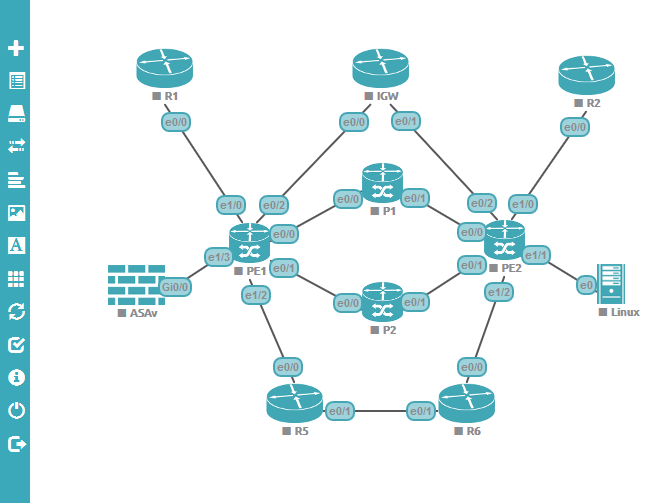
\includegraphics[width=0.75\textwidth]{unetlab_web}
    \caption{Webové rozhranie nástroja UNetLab}
    \cite{obr_unetlab_web}
    \label{obr:unetlab_web}
\end{figure}

\subsection{EVE-ng}

EVE-ng je simulačný nástroj sietí, ktorý vznikol ako klon a nasledovník nástroja UNetLab. Celkovou funkcionalitou, až na niektoré zmeny, napr. použitie MySQL namiesto SQLite, pridaná podpora pre ďalšie zariadenia), a vzhľadom webového rozhrania sa preto veľmi podobá na svojho predchodcu. Nástroj je postavený na platforme Linux a vyvíjaný prevažne v jazykoch JavaScript a PHP. Web rozhranie je realizované ako webová aplikácia s použitím framework nástroja \emph{Angular JS} a \emph{Twitter Bootstrap} \cite{eve_ng_technologies}.

EVE-ng sa v priebehu marca 2018 rozdelilo na tri verzie: Community, Professional a Learning Centre. Community verzia je open-source, aj keď \emph{gitlab} repozitár bol neprístupný pre verejnosť v priebehu novembra/decembra 2017. Napriek tomu sú na serveri všetky súbory prístupné a upravovateľné. Túto verziu je možné slobodne šíriť a upravovať. Verzia Professional obsahuje niektoré funkcionality, ktoré uľahčujú prácu s nástrojom, ale vývojári sa rozhodli spoplatniť ju. Learning Centre verzia obsahuje funkcionality na nasadenie do produkčného prostredia, ako je napr. rozdelenie používateľov do používateľských rolí. Podrobný zoznam podporovaných funkcii v jednotlivých verziách je dostupný v \cite{eve_ng_versions_table} a \cite{eve_ng_versions_list}.

Vzhľad webového rozhrania EVE-ng je znázornený na obrázku \ref{obr:eve_ng_web}. Rozdiely jednotlivých verzii EVE-ng sú znázornené v tabuľke \ref{tab:eve_ng_versions}.

\begin{figure}
    \centering
    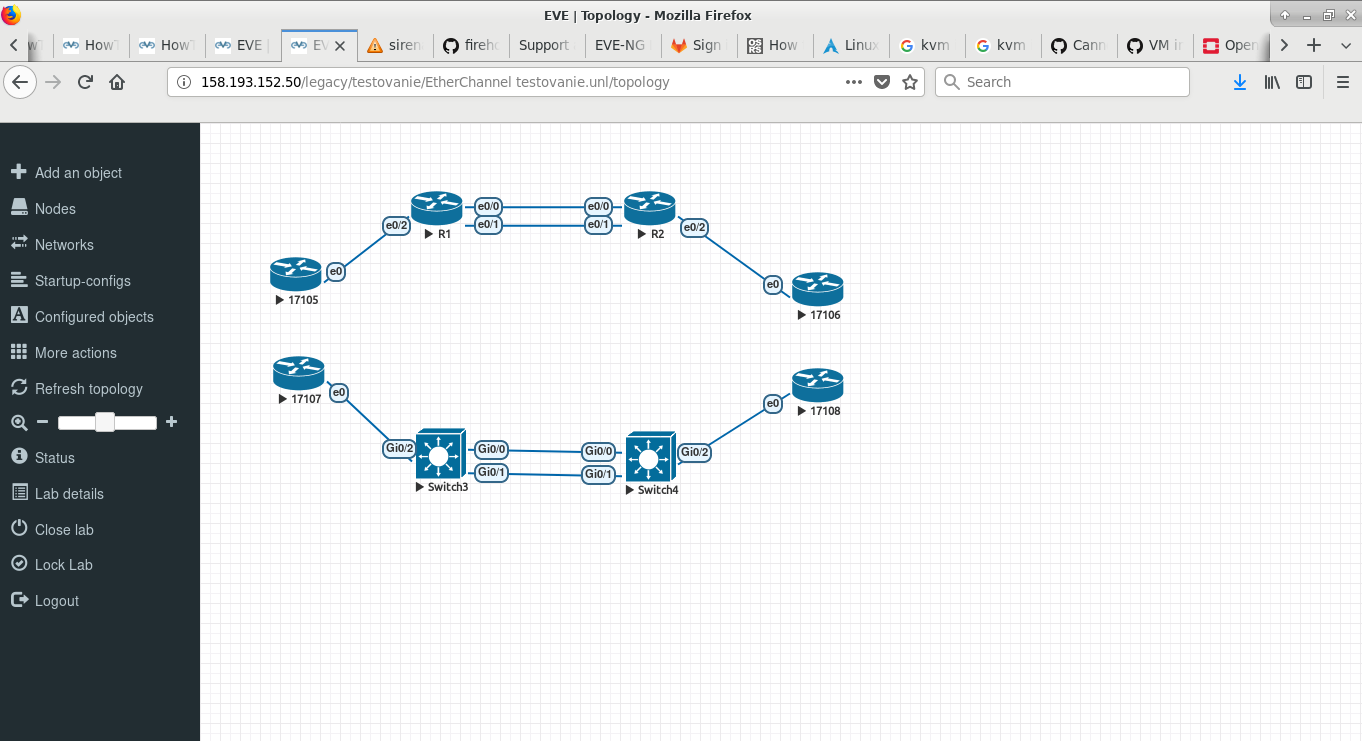
\includegraphics[width=0.75\textwidth]{eve_ng_web}
    \caption{Webové rozhranie nástroja EVE-ng}
    \label{obr:eve_ng_web}
\end{figure}

\begin{longtable}{| m{3cm} | m{2cm} | m{2cm} | m{2cm} | m{4cm} |}
\caption{Porovnanie EVE-ng verzii}
\label{tab:eve_ng_versions} \\
\hline
Features/Edition                                      & Community         & Professional    & Learning Center      & Description                                                                                                   \\ \hline
Price                                                 & Free              & 99 EUR w/o VAT  & 99 EUR + Added Roles &                                                                                                               \\ \hline
User's roles                                          & admin only        & admin only      & admin, user, editor  & Restrictions of the EVE usage, WEB UI, per user based                                                         \\ \hline
Lock user per folder                                  & No                & No              & Yes                  & User cannot see other EVE folders, only his own                                                               \\ \hline
Lock user edit rights                                 & No                & No              & Yes                  & User cannot edit labs, images etc                                                                             \\ \hline
Shared Lab Folder                                     & No                & No              & Yes                  & Shared lab folder visible for all users                                                                       \\ \hline
User's account validity ( 1/4 Hour accuracy )         & No                & No              & Yes                  & Ability to set calendar validity for account, Date and time ( From -\textgreater To )                         \\ \hline
Lab Timer                                             & No                & Yes             & Yes                  & Timer for Lab training                                                                                        \\ \hline
Running labs folder                                   & No                & Yes             & Yes                  & User can run more than one lab. Running labs will appear in special running labs folder. Per user based       \\ \hline
Node limit per lab                                    & 63                & 1024            & 1024                 & Limit of nodes to run per lab                                                                                 \\ \hline
TCP ports                                             & fixed 128 per POD & Dynamic 1-65000 & Dynamic 1-65000      & Automatic TCP port choose for telnet session                                                                  \\ \hline
Local Wireshark capture                               & Yes               & No              & No                   & Local wrapper using ssh and root password to the EVE                                                          \\ \hline
Local Telnet client                                   & Yes               & Yes             & Yes                  & Local wrapper using locally installed telnet client                                                           \\ \hline
Local VNC client                                      & Yes               & Yes             & Yes                  & Local wrapper using locally installed vnc client                                                              \\ \hline
Wireshark integrated                                  & No                & Yes             & Yes                  & Docker integrated wireshark                                                                                   \\ \hline
Docker container support                              & No                & Yes             & Yes                  & Docker container support                                                                                      \\ \hline
Running nodes interface connections (hot connections) & No                & Yes             & Yes                  & Hot/live nodes interface connection                                                                           \\ \hline
NAT Cloud                                             & No                & Yes             & Yes                  & Integrated NAT cloud, connect node to the internet. NAT to the EVE management interface DHCP 169.254.254.0/24 \\ \hline
HTML console without Wireshark capture                & Yes               & No              & No                   & HTML console                                                                                                  \\ \hline
HTML console with Wireshark capture                   & No                & Yes             & Yes                  & HTML wireshark capture                                                                                        \\ \hline
HTML Desktop Console                                  & No                & Yes             & Yes                  & Integrated Docker PC management                                                                               \\ \hline
Multi startup configuration choose per lab            & No                & Yes             & Yes                  & Option to create and boot lab from different startup configurations, multi startup config                     \\ \hline
Export/Import configs or config packs to local PC     & No                & Yes             & Yes                  & Option import and export single config or config packs to the lab                                             \\ \hline  
\end{longtable}

\subsection{GNS3}

GNS3, Graphical Network Simulator 3, je open-source sieťový simulátor sietí. Integruje všetky virtualizačné technológie najednom mieste: Dynamips, Cisco IOU aj zariadenia tretích strán (QEMU). Od verzie 1.5 sú v GNS3 podporované aj Docker kontajnery, čo je veľkou výhodou oproti iným nástrojom, pretože Docker kontajnery potrebujú menej systémových prostriedkov \cite{gns3_docker}.

GNS3 sa skladá z klientskej a serverovej časti. Klientská časť pozostáva z aplikácie \emph{GNS3 Client} a je celá napísaná v jazyku Python \cite{gns3_gui_github}. Klientská aplikácia je multiplatformová t.j. je kompatibilná s platformami Windows, Linux a macOS. Existuje aj klientská webová aplikácia \emph{gns3-web} \cite{gns3_web_github}.

Serverová časť môže byť realizovaná ako serverová aplikácia \emph{GNS3 Server}, ako virtuálny stroj \emph{GNS3 VM} alebo ako vzdialený server.

Serverová aplikácia \emph{GNS3 Server} sa spustí predvolene pri spustení klientskej aplikácie. Rovnako, ako GNS3 klientská aplikácia, aj serverová aplikácia je napísaná celá v jazyku Python \cite{gns3_server_github}.

GNS3 VM aj vzdialený server je postavený na platforme Linux. Vzdialený server nemusí nutne byť fyzický server, na ktorom je nasadený GNS3 server. Môže byť v ľubovoľnom virtualizačnom nástroji, napr. vo VMware. VMware je odporúčaná voľba pre tento virtualizačný nástroj, pretože podporuje vnorenú virtualizáciu, čo VirtualBox doposiaľ nepodporuje \cite{nested_virtualization}.

GNS3 VM resp. vzdialený server sa spravuje cez príkazový riadok. Používateľovi je dostupná klientská aplikácia. Portové čísla na vzdialený prístup sa zariadeniam prideľujú automaticky, avšak je možné manuálne meniť rozsah, v akom sa majú portové čísla automaticky prideľovať, dokonca umožňuje aj manuálnu zmenu čísla portu pre jednotlivé zariadenia \cite{gns3_console_ports, gns3_console_ports_remote}. Vzdialený prístup k zariadeniam v topológii je realizovaný protokolom \emph{telnet}, \emph{vnc} alebo\emph{rdp}. Topológie sa vytvárajú v klientskej aplikácii prepájaním uzlov medzi sebou pomocou myši. V predvolenom nastavení sú všetky topológie zdieľané a môže ich meniť ktokoľvek, kto má prístup k web rozhraniu, pretože v predvolenom nastavení nástroj nevie rozlišovať rôzne typy používateľov ani ich izolovať. Počet topológii, ktoré môžu byť súčasne spustené je obmedzené iba výkonom servera. Napriek tomu môžu na jednej topológii môžu pracovať aj viacerí študenti tým, že si otvoria rovnaký projekt na vzdialenom serveri. Zmeny v takejto zdieľanej topológii sa prejavia okamžite všetkým používateľom. Jeden používateľ môže mať spustených aj viacero topológii, v klientská aplikácia však dovoľuje pracovať iba s jednou naraz. Topológia sa dá kedykoľvek zatvoriť. Aj GNS3, podobne ako aj ďalšie nástroje, umožňuje prepojiť topológiu so živou sieťou pomocou \emph{bridge} rozhrania.

Vývoj tohto nástroja stále pokračuje. Na obrázku \ref{obr:gns3_client} je znázornená klientská aplikácia GNS3 Client.

\begin{figure}
    \centering
    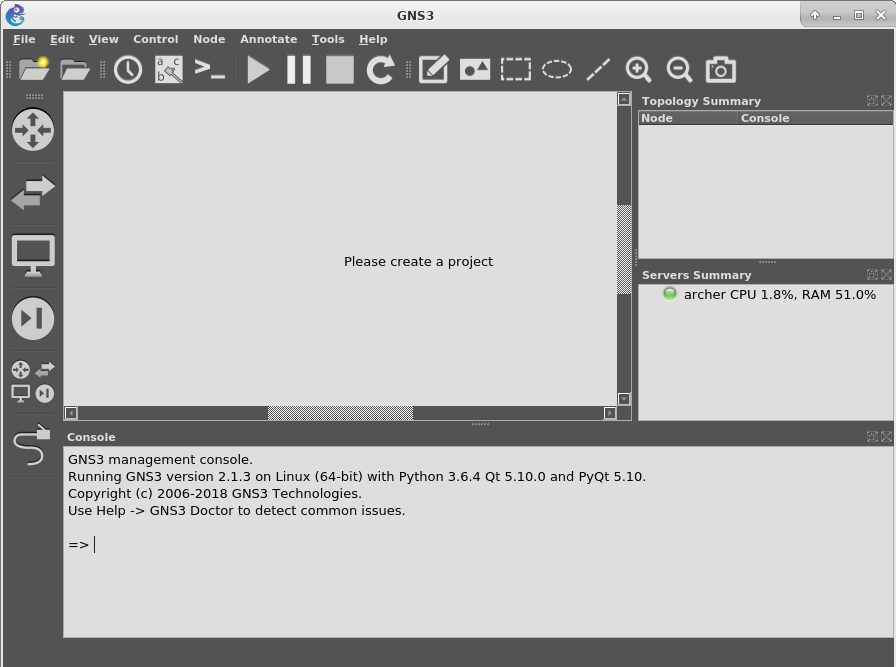
\includegraphics[width=0.75\textwidth]{gns3_client}
    \caption{Klientská aplikácia GNS3}
    \label{obr:gns3_client}
\end{figure}

\subsection{UNetLabv2}

UNetLabv2 je nasledovníkom nástroja UNetLab. Je postavený na platforme Docker kontajnerov. Jednotlivé úlohy sú distribuované naprieč kontajnermi. To zaisťuje lepšiu škálovateľnosť pri zachovaní rovnakej funkcionality. Zatiaľ ešte nie je verejne nedostupný.

Architektúra nástroja UNetLabv2 je znázornená na obrázku \ref{obr:unetlabv2_arch}

\begin{figure}
    \centering
    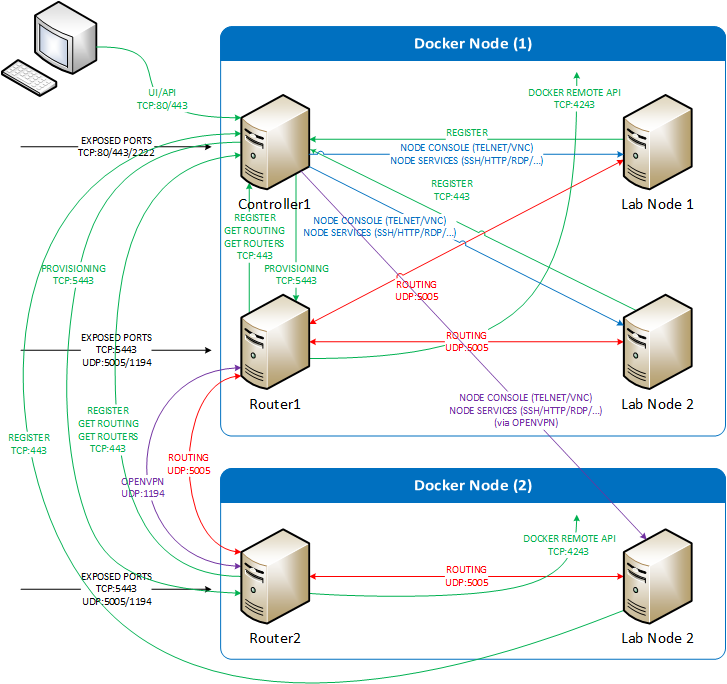
\includegraphics[width=0.75\textwidth]{unetlabv2_arch}
    \caption{Architektúra nástroja UNetLabv2} \cite{obr_unetlabv2_arch}
    \label{obr:unetlabv2_arch}
\end{figure}

\section{Vyhodnotenie}

Z vyššie uvedených nástrojov má zmysel zaoberať sa nástrojmi EVE-ng a GNS3 z nasledovných dôvodov:
\begin{itemize}
    \item Open-source vývoj oboch nástrojov umožňuje ich používanie bez poplatkov, obáv o porušenie licenčných podmienok a poskytuje možnosť upravovať ich podľa vlastných požiadaviek.
    \item Podpora zariadení od rôznych výrobcov.
    \item Jednoduché ovládanie.
\end{itemize}

V priebehu projektu sme sa preto zamerali na nástroje GNS3 a EVE-ng. Počas neho sa však ukázalo, že GNS3 nie je vhodná pre vzdialené použitie, preto sme sa týmto nástrojom ďalej nezaoberali. V čase skúmania bol nástroj GNS3 vo verzii 1.5.3. Keď sme skúšali použiť GNS3 ako vzdialený server, klientská aplikácia sa na GNS3 vzdialený server nevedela pripojiť, hoci sme postupovali podľa návodov na GNS3 stránke a pri testovaní nestála v pripojení na server žiadna prekážka napr. firewall.

GNS3 od vydania stabilnej verzie 2.0.0 opravila problém s nasadením ako vzdialený server. Avšak vtedy som už začal s hlbším skúmaním EVE-ng. Skúmanie dvoch nástrojov naraz do hĺbky by bolo časovo veľmi náročné. GNS3 slúžila počas skúmania ako podporný nástroj pre pochopenie rôznych technických súčastí virtualizácie sieťových zariadení.

Vo zvyšku diplomovej práce sa zaoberám nástrojom EVE-ng a jeho nasadením do vyučovania na katedre.
